\documentclass[conference]{IEEEtran}
\IEEEoverridecommandlockouts
% The preceding line is only needed to identify funding in the first footnote. If that is unneeded, please comment it out.
\usepackage{cite}
\usepackage[T1]{fontenc}
\usepackage{amsmath,amssymb,amsfonts}
\usepackage{graphicx}
\usepackage{textcomp}
\usepackage{xcolor}
\usepackage{titlesec}
\usepackage{textcomp}
\usepackage{epsfig}
\usepackage{algpseudocode}
\usepackage{pgfplots}
\usepackage{tikz}
\usepackage{hyperref}
\pgfplotsset{width=10cm,compat=1.9}
 \usepgfplotslibrary{external}



\usepackage[linesnumbered,ruled,vlined]{algorithm2e}
\def\BibTeX{{\rm B\kern-.05em{\sc i\kern-.025em b}\kern-.08em
    T\kern-.1667em\lower.7ex\hbox{E}\kern-.125emX}}

\usepackage[ruled,vlined]{algorithm2e}

\tikzexternalize 
\begin{document}

\title{ Optimising Binary Search Using Heuristics\\
\text{\Large{DAA ASSIGNMENT-3 , GROUP 7}}
}
\author{\IEEEauthorblockN{Medha Balani}
\IEEEauthorblockA{ \text{IIT2019021}}
\and
\IEEEauthorblockN{Saksham Aggarwal}
\IEEEauthorblockA{ \text{IIT2019022}}
\and
\IEEEauthorblockN{Utkarsh Gangwar}
\IEEEauthorblockA{ \text{IIT2019023}}
}

\maketitle
\paragraph{\textbf{\textit{Abstract: In this paper we have described an algorithm that is an improved version of binary search using heuristics . This   algorithm optimizes the worst and average case of binary search algorithm . We have also done the apriori and aposteriori analysis of our algorithm. }}}\\

\section{INTRODUCTION}\\
Searching Algorithms are used to check for
an element in a data structure or retrieve its information if it exists.Search algorithms can be classified based on their mechanism of searching. \\Linear search algorithms check every record for the one associated with a target key in a linear fashion. \\Binary searches, repeatedly target the center of the search structure and divide the search space into half. \\Comparison search algorithms improve on linear searching by successively eliminating records based on comparisons of the keys until the target record is found, and can be applied on data structures with a defined order. \\Finally, hashing directly maps keys to records based on a hash function. 
\\Heuristic is a technique designed for solving a
problem more quickly when trivial methods are
too slow, or for finding an approximate solution
when trivial methods fail to find any exact
solution.
\\Binary search is the most popular Search algorithm.It is efficient and also one of the most commonly used techniques that is used to solve problems.

If all the names in the world are written down together in order and you want to search for the position of a specific name, binary search will accomplish this in a maximum of 35 iterations.

Binary search works only on a sorted set of elements. To use binary search on a collection, the collection must first be sorted.

When binary search is used to perform operations on a sorted set, the number of iterations can always be reduced on the basis of the value that is being searched.

\section{ALGORITHM DESIGN}
\subsection{Problem Statement}
 We are required to return the index of the element \(key\) in the array \(Arr\) which is sorted in non-decreasing order.We return -1 if \(key\) doesn't occur in \(Arr\).
\subsection{Algorithm Description}
Similar to the binary search algorithm we initialise the lower bound $l = 0 $(lowest index in the array \(Arr\)) and Upper bound $r = n-1$ (where \(n\) is the size of array \(Arr\)).

In binary search we repeatedly compared the middle element of our search space with the given \(key\)
, this indicates that if the key is present in the left or right end of the array \(Arr\) binary search would take comparatively more iterations to find it out than it would take if element is in the middle part of the array \(Arr\).

In this algorithm we not only compare the middle element of our search space with \(key\) but also compare \(key\) with left and right bounds , so that we don't take many iterations to find elements present at the ends.

Similar to Binary Search we reduce our search space to half based on the comparison between the values of \(key\) and element present at middle in the array \(Arr\).


 \subsection{Pseudo-code}  
\begin{algorithm}[H] 
    \caption{Optimised Binary search}
    \KwIn{Sorted Array \(Arr\) of size $n$ and \(key\)}
    \KwOut {Index of \(key\)}
    \DontPrintSemicolon
    \SetKwFunction{FMain}{OptimisedBinarySearch}
    \SetKwProg{Fn}{Function}{:}{}
    \Fn{\FMain{$Arr$,$n$,$key$}}{
        
       $l \gets 0\;$\\
       $r \gets n-1\;$\\
       $Ans \gets -1\;$\\
       
    \While{$l \leq r$}{
        
        $mid \gets l + \frac{(r-l)}{2}\;$
        
        \If{$Arr[l] = key$}{
            $Ans \gets l\;$
            \\ \KwRet Ans\; 
        }
        \If{$Arr[r] = key$}{
            $Ans \gets r\;$
             \\\KwRet Ans\; 
        }
        \If{$Arr[mid] = key$}{
            $Ans \gets mid\;$
            \\ \KwRet Ans\; 
        }
        \If{$Arr[mid] < key $}{
            $l \gets mid+1\;$
        }
        \Else{
            $r \gets mid-1\;$
        }
    }
     \KwRet Ans\;
        
    }
\end{algorithm}
\section{ALGORITHM ANALYSIS}

\subsection{Apriori Analysis}

\begin{tabular}{ |p{2cm}||p{1cm}|p{1cm}|p{2cm}|  }
 \hline
 \multicolumn{4}{|c|}{Table : Time Complexity} \\
 \hline
 Steps & Time &Best Freq. &Freq.\\
 \hline
  2,3,4 & 3 & 1 & 1\\
  \hline
  5 & 1 & 1 & $logN$\\
  \hline
  6 & 3 & 1 & $logN$\\
  \hline
  7,8,9 & 4 & 1 & $logN$\\
  \hline
  10,11,12 & 4 & 1 & $logN$\\
  \hline
  13,14,15 & 4 & 1 & $logN$\\
  \hline
  16 & 1 & 0 & $logN$\\
  \hline
  17 & 2 & 1 & $logN$\\
  \hline
  18 & 1 & 0 & $logN$\\
  \hline
  19 & 2 & 1 & $logN$\\
 \hline
\end{tabular}

From the above table we can say that best case for this algorithm would be when \(key\) is present at either of mid , end or start of the array \(Arr\).

$T_{\Omega} \propto 3 \ast 1 + 1 \ast 1 +3 \ast 1 + 4 \ast 1 + 4 \ast 1 + 4 \ast 1 + 1 \ast 0 + 2 \ast 1 +  1 \ast 0 + 2 \ast 1 $\\\\
$T_{\Omega} = \Omega(1)$

While in the worst Case : 
 
 $T_{O} \propto 3 \ast 1 + 1 \ast logN +3 \ast logN + 4 \ast logN + 4 \ast logN + 4 \ast logN + 1 \ast logN + 2 \ast logN +  1 \ast logN + 2 \ast logN $\\\\
 $T_{O} \propto 3 + 21 \ast logN$\\\\
 $T_{O} = O( logN )$
 
\subsection{Space Complexity}
Since no extra space is used in this algorithm , so auxiliary space is constant.
Only the input array is of size n. So , Space Complexity = Input Space + Auxiliary Space  = O(n), this Algorithm uses linear Space .
\section{EXPERIMENTAL STUDY}
\subsection{Graph-1}
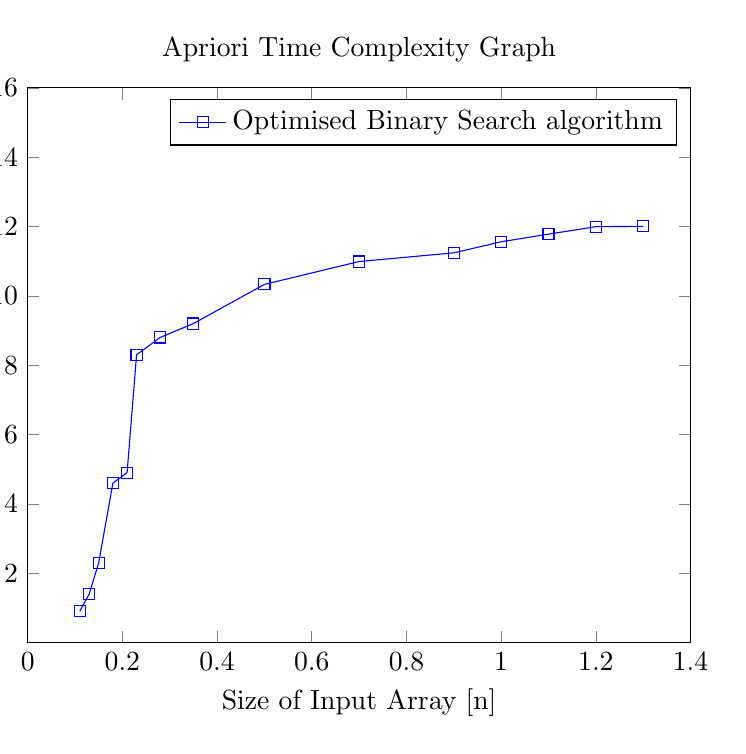
\begin{tikzpicture}[trim left=0cm]

\begin{axis}[
    title={Apriori Time Complexity Graph},
    xlabel={Size of Input Array [n]},
    ylabel={Time(in microseconds) [t]},
     xmin=0, xmax=1.4,
    ymin=0, ymax=16,
    xtick={0,0.2,0.4,0.6,0.8,1.0,1.2,1.4},
    ytick={2,4,6,8,10,12,14,16}
]

\addplot[
    color=blue,
    mark=square,
    ]
    coordinates {
   (0.11,0.9)(0.13,1.4)(0.15,2.3)(0.18,4.6)(0.21,4.9)(0.23,8.3)(0.28,8.8)(0.35,9.2)(0.5,10.33)(0.7,10.99)(0.9,11.24)(1,11.56)(1.1,11.78)(1.2,11.996)(1.3,12.005)
    };
    \legend{Optimised Binary Search algorithm}
   \end{axis}
   
\end{tikzpicture}
\linebreak\linebreak\linebreak\linebreak
\subsection{Graph-2}
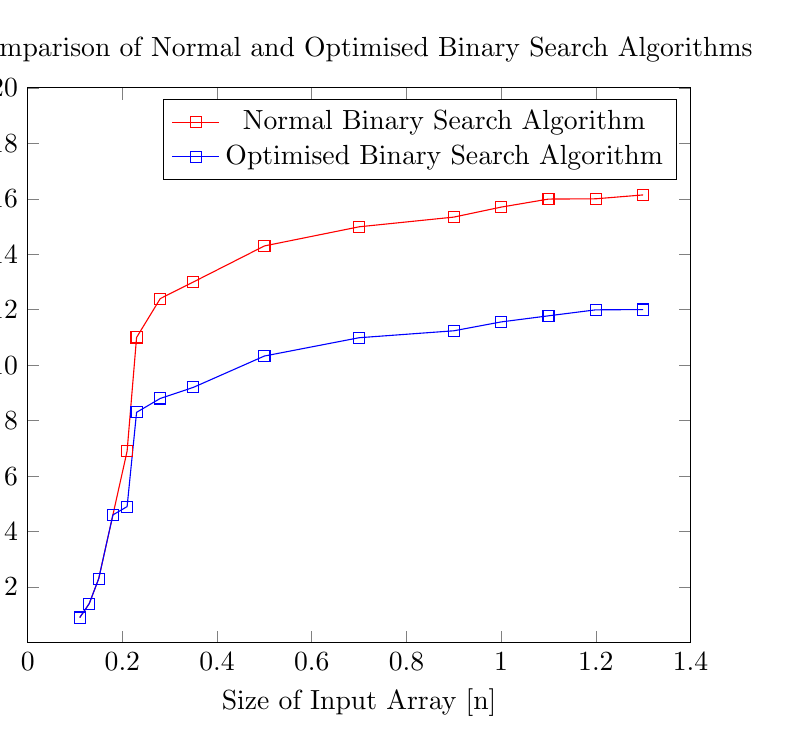
\begin{tikzpicture}[trim left=0cm]
\begin{axis}[
    title={Comparison of Normal and Optimised Binary Search Algorithms},
    xlabel={Size of Input Array [n]},
    ylabel={Time(in microseconds) [t]},
     xmin=0, xmax=1.4,
    ymin=0, ymax=20,
    xtick={0,0.2,0.4,0.6,0.8,1.0,1.2,1.4},
    ytick={2,4,6,8,10,12,14,16,18,20}
]

\addplot[
    color=red,
    mark=square,
    ]
    coordinates {
    (0.11,0.9)(0.13,1.4)(0.15,2.3)(0.18,4.6)(0.21,6.9)(0.23,11)(0.28,12.4)(0.35,13)(0.5,14.3)(0.7,14.99)(0.9,15.34)(1,15.7)(1.1,15.99)(1.2,16)(1.3,16.14)
    };
    \legend{$Optimised Binary Search algorithm$}
  
   
\addplot[
    color=blue,
    mark=square,
     ]  
     coordinates {
    (0.11,0.9)(0.13,1.4)(0.15,2.3)(0.18,4.6)(0.21,4.9)(0.23,8.3)(0.28,8.8)(0.35,9.2)(0.5,10.33)(0.7,10.99)(0.9,11.24)(1,11.56)(1.1,11.78)(1.2,11.996)(1.3,12.005)
    };
    \legend{Normal Binary Search Algorithm,Optimised Binary Search Algorithm}
    
    
   \end{axis}
     
   
\end{tikzpicture}

From the above graphs we can conclude that by using heuristics we can optimise binary search algorithm in the worst case as well as average case.\\Also the graphs are consistent with the apriori analysis.


\section{ILLUSTRATION}
Let the given array be: \{5,10,17,30,35,65,80,120,150,200\}
Key is the element to be searched\\\\
\textbf{Case 1 : Element is at first or last position}\\\\
    Key = 200\\
\textbf{Using Binary Search -}\\
\textbf{First iteration:} low =0 high =9 mid =4 a[4] =35\textless 200
\\low= mid+1 =5\\
\textbf{Second iteration:} low =5 high =9 mid =7 a[7] =120\textless 200 
\\low= mid+1 =8\\
\textbf{Third iteration:} low =8 high =9 mid =8 a[8] =150\textless 200 
\\low= mid+1 =9\\
\textbf{Fourth iteration:} low =9 high =9 mid =9 a[9] =200 == Key,   
\\Total iterations = 4\\
\textbf{Using improved Binary Search -}\\
\textbf{First iteration:} low = 0 , high = 9 mid =4
\\a[high]= 200  ==  key\\
Total iterations = 1\\\\
\textbf{Case 2 : Element present in first half}\\\\
   Key = 30\\
\textbf{Using Binary Search -}\\
\textbf{First iteration:} low = 0 , high = 9 mid =4\\
a[4] =35 >30 
\\high = mid -1 = 3\\
\textbf{Second iteration:} low =0 high =3 mid = 1
\\a[1]=10<30
\\low =mid +1= 2\\
\textbf{Third iteration:} low =2 high =3 mid = 2
\\a[2] = 17 < 30 
\\low  = mid +1 = 3\\
\textbf{Fourth iteration:} low =3 high=3 mid = 3
\\a[3]=30 == Key
\\Total iterations =4\\
\textbf{Using Improved  Binary Search -}\\
\textbf{First iteration:} low = 0 , high = 9 mid =4
\\a[4]=35 >30 
\\high = mid -1= 3  low =low +1\\
\textbf{Second iteration:} low = 1 high = 3 mid = 2
\\a[high]=30 ==Key
\\Total iteration = 2





\section{CONCLUSION}
The above proposed algorithm improves traditional binary search algorithm by eliminating redundant iterations by adding a few if statements to also check at left and right bounds along-with the middle element.But the overall complexity of the algorithm still remains O($logN$).

\section{REFERENCES}
\begin{enumerate}
    \item \url{https://www.hackerearth.com/practice/algorithms/searching/binary-search/tutorial/}
    \item \url{https://en.wikipedia.org/wiki/Heuristic_(computer_science)}
\end{enumerate}

\end{document}
